\chptr{Problemi sui Grafi}


\section{Individuare un isomorfismo}
Consideriamo il problema seguente:
\begin{center}
Dati due o più grafi, si desidera stabilire se sono tra loro isomorfi.
\end{center}
Quando si affronta un problema come questo, spesso torna utile ricorrere
alle proprietà mostrate di seguito.
\begin{tcolorbox}[colback=red!30, colframe=red!30!black, title=Alcune caratteristiche dei grafi isomorfi]
Siano $G,G'$ grafi finiti. Supponiamo $G\cong G'$. Allora:
\begin{enumerate}
\item $\text{Score}(G)=\text{Score}(G')$.
\item $G,G'$ hanno lo stesso numero di componenti connesse.
\item $G$ è 2-connesso $\Longleftrightarrow$ $G'$ è 2-connesso.
\item $G$ è hamiltoniano $\Longleftrightarrow$ $G'$ è hamiltoniano.
\item $G,G'$ hanno lo stesso numero di sottografi che sono $k$-cicli.
\item Sia $f:V\to V'$ un isomorfismo. Sia $v\in V$ tale che $\deg_G(v)=k\in\mathbb{N}$.
Siano $v_1,...,v_k \in V$ adiacenti a $v$. Allora $f(v_1),...,f(v_k)$ sono
adiacenti a $f(v)$: \[\deg_G(v)=\deg_G(f(v)) \quad \deg_G(v_i)=\deg_G(f(v_i)) \quad \forall i \in\{1,...,k\}\]
\end{enumerate}
\end{tcolorbox}

La proprietà (6) potrebbe essere la più complessa da applicare. Intuitivamente,
essa permette di trovare grafi tra loro non isomorfi osservando i gradi
di vertici tra loro adiacenti. Un sempio di applicazione di (6) è presente
in uno degli esercizi di esempio mostrati in questa sezione.
\\\\
Supponiamo di avere $G,G'$ grafi finiti. Per stabilire se sono isomorfi, si
controllano le proprietà da (1) a (6). Se anche una sola è falsa, allora
si può concludere con certezza che $G\not\cong G'$. Altrimenti non si può
ancora dare una risposta: infatti si tratta di condizioni sufficienti ma
non necessarie all'esistenza di isomorfismi. Si prova allora a definire un
isomorfismo "a mano".

\newpage
\begin{tcolorbox}[enhanced, breakable, colback=blue!30, colframe=blue!30!black, title=Esempio]
Siano rispettivamente $G_1, G_2, G_3$ i grafi raffigurati qui sotto.
Si dica, motivando la risposta, quali tra essi sono isomorfi e quali no.
\begin{figure}[H]
\centering
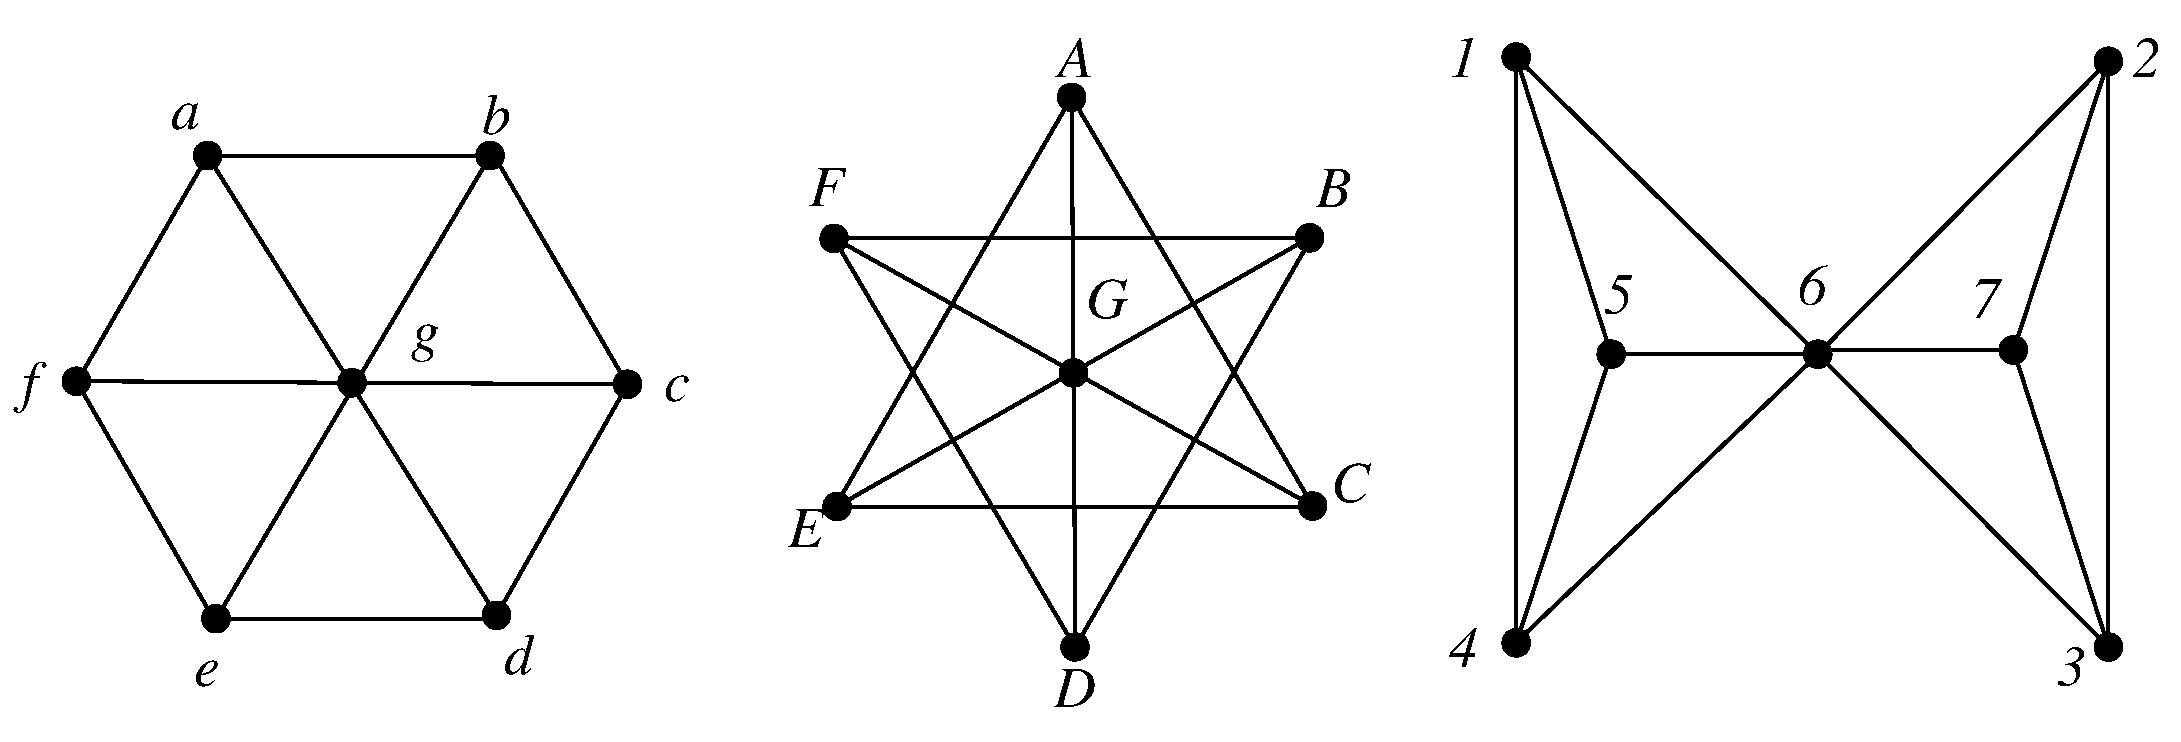
\includegraphics[scale=0.27]{figures/exisomorph.pdf}
\end{figure}
\textit{Soluzione:} verifichiamo prima le condizioni necessarie per l'esistenza
di isomorfismi tra grafi finiti:
\begin{enumerate}
    \item $\text{Score}(G_1) = \text{Score}(G_2) = \text{Score}(G_3)$: nulla si può dire.
    \item In ciascuno dei tre grafi, ogni coppia di vertici può essere collegata con passeggiate. Dunque $G_1,G_2,G_3$ sono connessi: nulla si può dire.
    \item Osserviamo che $(a,b,c,d,e,f,g,a)$ è un ciclo hamoltoniano in $G_1$.
    Dunque $G_1$ è un grafo hamiltoniano e quindi anche 2-connesso. Possiamo inoltre
    notare che $G_2 - G$ e $G_3 - 6$ non sono connessi, quindi $G_2$ e $G_3$ non
    sono grafi 2-connessi. Possiamo concludere che
    \[ G_1 \not\cong G_2 \quad \text{ e } \quad G_1 \not\cong G_3 \]
    \item Dal punto precedente abbiamo concluso che $G_2$ e $G_3$ non sono 2-connessi,
    dunque nemmeno hamiltoniani: nulla si può dire su questi due grafi.
    \item $G_2$ e $G_3$ hanno lo stesso numero di 3-cicli: nulla si può dire.
    \item Notiamo che $G_2$ e $G_3$ hanno un unico vertice di grado massimo:
    $G\in V(G_2)$ e $6 \in V(G_3)$ con $\deg_{G_2}(G) = \deg_{G_3}(6) = 6$.
    Dunque, se esistesse un isomorfismo $f:V(G_2)\to V(G_3)$, allora $f(G) = 6$.
    Osserviamo che $G$ è adiacente a sei vertici, ciascuno di grado 3. D'altra parte,
    anche $6$ è adiacente a sei vertici, ciascuno con grado 3. Non si deduce alcuna
    contraddizione: nulla si può dire.
\end{enumerate}
Non concludendo ancora nulla su $G_2$ e $G_3$, proviamo a definire un isomorfismo
tra questi grafi. Sia:
\begin{align*}
    V(G_2) &\stackrel{f}{\to} V(G_3)\\
    A&\mapsto 2\\
    B&\mapsto 5\\
    C&\mapsto 7\\
    D&\mapsto 4\\
    E&\mapsto 3\\
    F&\mapsto 1\\
    G&\mapsto 6
\end{align*}
Poiché nella colonna di destra appaiono tutti i vertici di $G_3$ senza ripetizioni,
la funzione $f:V(G_2)\to V(G_3)$ è una bigezione. Verifichiamo se si tratta anche
di un morfismo da $G_2$ a $G_3$:
\begin{align*}
    E(G_2) &\stackrel{'f'}{\to}\binom{V(G_3)}{2}\\
    \{A,E\} &\mapsto \{2,3\}\\
    \{A,G\} &\mapsto \{2,6\}\\
    \{A,C\} &\mapsto \{2,7\}\\
    \{E,C\} &\mapsto \{3,7\}\\
    \{E,G\} &\mapsto \{3,6\}\\
    \{C,G\} &\mapsto \{7,6\}\\
    \{F,B\} &\mapsto \{1,5\}\\
    \{F,G\} &\mapsto \{1,6\}\\
    \{F,D\} &\mapsto \{1,4\}\\
    \{D,G\} &\mapsto \{4,6\}\\
    \{D,B\} &\mapsto \{4,5\}\\
    \{B,G\} &\mapsto \{5,6\}\\
\end{align*}
Segue che $f(E(G_2)) \subseteq E(G_3)$, dunque $f$ è un morfismo da $G_2$ a $G_3$.
D'altra parte i lati di $G_3$ che compaiono nella seconda colonna della precedente
lista sono tutti i 12 lati di $G_3$. Allora $f(E(G_2)) = E(G_3)$, ovvero $f$ è un
isomorfismo da $G_2$ a $G_3$. Dunque $G_2 \equiv G_3$.

\end{tcolorbox}



\newpage
\section{Riconoscere uno score}
Si consideri il seguente problema:
\begin{center}
dato $d = (d_1,...,d_n)\in\mathbb{N}^n$, stabilire se esiste un grafo $G$
tale che $\text{Score}(G)=d$
\end{center}
Presentiamo ora un ridottissimo numero di lemmi, o \textit{ostruzioni}, che
consentono di verificare se un vettore di interi può \emph{non} essere lo score
di un grafo. Si sottolinea che:
\begin{itemize}
\item Le ostruzioni sono \textit{condizioni sufficienti ma non
necessarie} all'esistenza di un grafo: dato un vettore $d$, se
anche tutte le ostruzioni mostrate qui fallissero, non
si potrebbe dire alcunché sull'esistenza di un grafo con score
$d$.

\item Alcune ostruzioni non sono applicabili a tutti i vettori:
ciò non implica la non esistenza di un possibile grafo con score
$d$.

\item Queste non sono le uniche ostruzioni esistenti: in base
alle dimensioni e alla conformazione del vettore dato, potrebbero
anzi esistere migliaia di ostruzioni applicabili.
\end{itemize}

\begin{tcolorbox}[colback=red!30, colframe=red!30!black, title=Ostruzione 1]
Sia $d=(d_1,...,d_n)\in\mathbb{N}^n, n\geq1, d_1\leq...\leq d_n$.
\[ d_n > n-1 \Longrightarrow \nexists G:\text{Score}(G)=d \]
\end{tcolorbox}

\begin{tcolorbox}[colback=blue!30, colframe=blue!30!black, title=Esempio: applicazione della prima ostruzione]
Viene dato $d=(1,1,1,2,2,3,4,8)$. Quindi $n=8,d_n=8$
ma $d_n = 8 > n - 1 = 8 - 1 = 7$. Quindi non esiste nessun grafo con
score $d$.
$\\\\$
\textbf{Motivazione:} non può esistere un grafo con tale score,
perché sono previsti $n$ vertici e ognuno di essi può essere
collegato ad al più $n-1$ vertici (ovvero può appartenere ad
al più $n-1$ lati).
\end{tcolorbox}

\begin{tcolorbox}[colback=red!30, colframe=red!30!black, title=Osservazione]
Sia $d=(0,...,0,d_1,...,d_n)\in\mathbb{N}^{n+m}$, dove compaiono
$m$ zeri e vale $0<d_1\leq...\leq d_n$. Sia $d'=(d_1,...,d_n)\in\mathbb{N}^n$.
\[ d \text{ è lo score di un grafo } \Longleftrightarrow d' \text{ è lo score di un grafo} \]
\end{tcolorbox}

\begin{tcolorbox}[colback=blue!30, colframe=blue!30!black, title=Esempio]
Viene dato $d=(0,0,0,1,1,2,2,2,3,4,9)$. L'ostruzione
1 non è verificata, quindi non si può ancora dare una risposta.
Estraiamo da $d$ lo score $d'=(1,1,2,2,2,3,4,9)$ e riapplichiamo
l'ostruzione: $d_n=9>n-1=8-1=7$. Segue che $d'$ non può rappresentare
lo score di un grafo e per l'Osservazione non lo è nemmeno $d$.
\end{tcolorbox}


\begin{tcolorbox}[colback=red!30, colframe=red!30!black, title=Ostruzione 2]
Siano $h,k\in\mathbb{N}\setminus\{0\}$, sia $n:=h+k$ e $d\in\mathbb{N}^n$
tale che $d=(d_1,...,d_h,n-1,...,n-1)$ dove $n-1$ compare $k$ volte
e $d_1\leq...\leq d_h < n-1$.
\[ d_1<k \Longrightarrow \nexists G:\text{Score}(G)=d \]
\end{tcolorbox}
\begin{tcolorbox}[colback=blue!30, colframe=blue!30!black, title=Esempio]
Viene dato $d=(1,2,3,4,5,6,7,8,8)$. L'ostruzione 1
non fornisce informazioni. Notiamo che è applicabile l'ostruzione 2:
$d_1=1<2$ quindi non esistono grafi con score $d$.
\end{tcolorbox}

\noindent Una motivazione verbale esaustiva può essere la seguente:
\emph{non può esistere un grafo con tale score,
perché sarebbero previsti $n$ vertici di cui $k$ collegati a
tutti gli altri, quindi $d_1$ dovrebbe valere almeno $k$.}

\begin{tcolorbox}[colback=blue!30, colframe=blue!30!black, title=Esempio: combinare l'osservazione alle altre ostruzioni]
Viene dato $d=(0,0,0,2,3,3,3,3,3,3,4,10,10,10)$.
\begin{enumerate}
\item $d_n=10 \not> n-1=14-1=13$: l'ostruzione 1 non fornisce
informazioni.

\item Non è applicabile l'ostruzione 2. Però il vettore $d'$
è valido, quindi applichiamo l'osservazione: $d'_1=2<3$, quindi
$d'$ non è lo score di un grafo e pertanto nemmeno $d$.
\end{enumerate}
\end{tcolorbox}  




\begin{tcolorbox}[colback=red!30, colframe=red!30!black, title=Ostruzione 3]
Sia $n\in\mathbb{N},n\geq3$. Sia $d=(d_1,...,d_n)\in\mathbb{N}^n,
d_1\leq...\leq d_n$. Definiamo: $L:=\left|\left\{ i\in\{1,...,n-2\}|d_i\geq2 \right\}\right|$.
\[ L < d_{n-1}+d_n-n \Longrightarrow \nexists G:\text{Score}(G)=d \]
\end{tcolorbox}

\begin{tcolorbox}[colback=blue!30, colframe=blue!30!black, title=Esempi]
Viene dato $d=(1,1,1,3,5,5,7,7,8,8)$.
\begin{enumerate}
\item $d_n=8>n-1=10-1=9$: nulla si può dire.
\item Ostruzione 2 non applicabile.
\item $L=5 < d_n+d_{n-1}-n=8+8-10 = 6 \Longrightarrow \nexists G:\text{Score}(G)=d$.
\end{enumerate}
Viene dato $d=(2,2,2,2,3,3,3,5,6)$.
\begin{enumerate}
\item $d_n=6>n-1=9-1=8$: nulla si può dire.
\item Ostruzione 2 non applicabile.
\item $L=7<5+6-9=2$: nulla si può dire.
\end{enumerate}
\end{tcolorbox}  

\begin{tcolorbox}[colback=red!30, colframe=red!30!black, title=Ostruzione 4]
Si veda il \textbf{lemma delle strette di mano}.
\[ d \text{ non soddisfa il lemma delle strette di mano} \Longrightarrow \nexists G:\text{Score}(G)=d \]
\end{tcolorbox}



\newpage
\section{Il teorema dello score}
Una volta verificato che il vettore fornito non soddisfa alcuna ostruzione,
è possibile procedere con l'applicazione del teorema dello score, che
rappresenta un buon metodo di verifica e costruzione di un possibile grafo
con score dato.
\begin{tcolorbox}[title=Teorema dello Score]
Sia $n\geq2$ e sia $d=(d_1,...,d_n)\in\mathbb{N}^n$ tale che $d_1\leq...\leq d_n\leq n-1$.
Definiamo $d'=(d'_1,...,d'_{n-1})\in\mathbb{N}^{n-1}$ ponendo:
\begin{align*}
d'_i:=
\begin{cases}
    d_i   & i<n-d_n\\
    d_i-1 & i\geq n-d_n
\end{cases}
\end{align*}
Allora $d$ è lo score di un grafo se e solo se lo è $d'$.
\end{tcolorbox}

\noindent Si noti che il teorema dello score incorpora già in sé la condizione
dell'ostruzione 1. La proprietà più apprezzabile di questo teorema
risiede nel fatto che esso fornisce un algoritmo che abbassa la
complessità dello score fornito, riducendolo ad una serie di casi
possibili trattabili con molta facilità. Il lemma seguente ci mostra
quali sono questi casi.

\begin{tcolorbox}[enhanced, breakable, colback=red!30, colframe=red!30!black, title={Casi notevoli dopo l'applicazione del teorema dello score}]
Sia $n\in\mathbb{N}\setminus\{0\}$ e sia $d=(d_1,...,d_n)\in\mathbb{N}^n$
tale che $d_1\leq...\leq d_n\leq 2$. Valgono:
\begin{enumerate}
\item Se $d=(0,...,0,2)$ oppure $n\geq 2$ e $d=(0,...,0,2,2)$ allora
non esiste un grafo con score $d$.

\item Se $d=(0,...,0)$ o $d=(0,...,0,2,2,...,2)$ ($m\geq 3$ elementi
di grado 2) allora esiste un grafo con tali score: $G_1$ con tutti
i vertici isolati, $G_2$ con $n-m$ vertici isolati e un $m$-ciclo.

\item Supponiamo che compaia almeno una volta l'unità 1. Se il numero
di volte in cui compare 1 è dispari, allora non esiste $G$ con tale
score (conseguenza del lemma delle strette di mano).

\item Supponiamo che 1 compaia in numero pari $2k+2\geq 2$ ($k\geq 0$),
che il numero di 0 sia $h\geq0$ e i 2 in numero $m\geq0$:
\[ d=(0,...,0,1,1,...,1,1,2,...,2) \]
Allora il seguente grafo $G$ ha score $d$:
\begin{figure}[H]
\centering
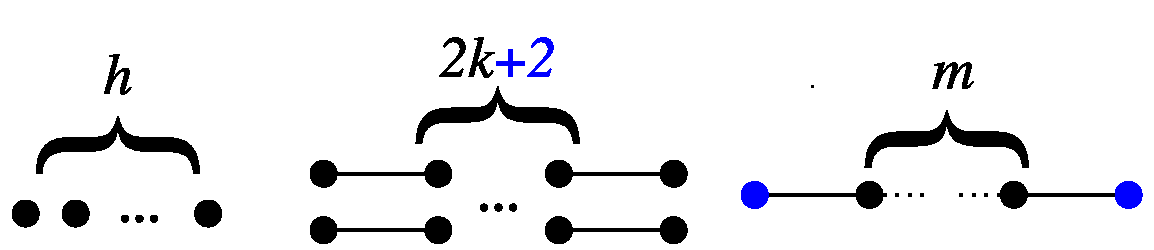
\includegraphics[scale=0.4]{figures/base.pdf}    
\end{figure}
\end{enumerate}
\end{tcolorbox}


\begin{tcolorbox}[enhanced, breakable, colback=blue!30, colframe=blue!30!black, title={Esempio di applicazione del teorema dello score}]
Stabilire se esiste un grafo con score $d=(2,2,2,2,3,3,3,5,6)$. In caso affermativo,
costruire un possibile grafo con score $d$, mediante il teorema dello score.
$\\\\$
\textit{Soluzione:} Passiamo in rassegna le ostruzioni viste finora:
\begin{enumerate}
    \item Osserviamo che $6>9-1$: nulla si può dire.
    \item Questa ostruzione non è applicabile: nulla si può dire.
    \item $L=7<5+6-9 = 2$: nulla si può dire.
    \item $d$ soddisfa il lemma dell strette di mano: nulla si può dire.
\end{enumerate}
Non avendo concluso nulla, ricorriamo al teorema dello score (sappiamo già dall'ostruzione 1
che il teorema è applicabile a $d$).
\begin{center}
    \begin{tabular}{c|lllllllll}
        $d$   & 2 & 2 & \textcolor{white}{2} & \textcolor{white}{2} & \textcolor{white}{3} & \textcolor{white}{3} & \textcolor{white}{3} & \textcolor{white}{5} & \textcolor{yellow}{6}\\
        \hline
        $d'$  & 2 & 2 & 1 & 1 & 2 & 2 & 2 & 4 & $\times$\\
              & 1 & 1 & 2 & \textcolor{white}{2} & \textcolor{white}{2} & \textcolor{white}{2} & \textcolor{white}{2} & \textcolor{green}{4} & \tiny{ordinato}\\
        \hline
        $d''$ & 1 & 1 & 2 & 1 & 1 & 1 & 1 & $\times$ &\\
              & 1 & 1 & 1 & 1 & \textcolor{red}{1} & \textcolor{red}{1} & \textcolor{red}{2} & & \tiny{ordinato}
    \end{tabular}
\end{center}
Ci siamo ricondotti ad una forma notevole dello score, facilmente
rappresentabile. Costruiamo $G''$, che ha score $d''$:
\begin{figure}[H]
\centering
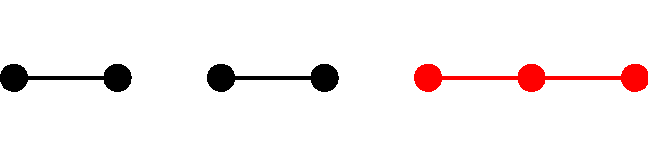
\includegraphics[scale=0.4]{figures/basescore.pdf}    
\end{figure}
Per il teorema dello score, sono score di qualche grafo anche $d'$ e
$d$. Costruiamo un grafo $G$ con score $d$ mediante il teorema dello score:
\begin{figure}[H]
\centering
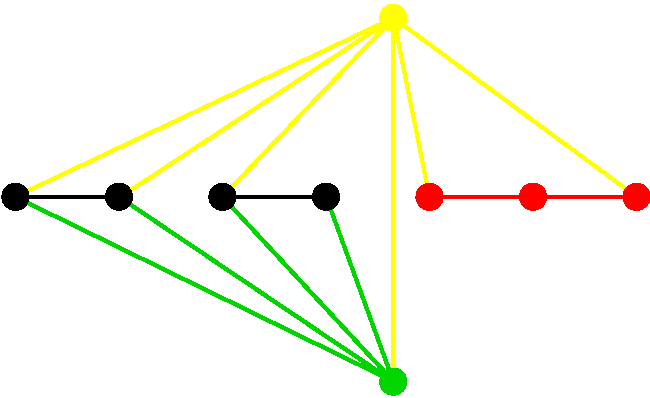
\includegraphics[scale=0.4]{figures/teoscore.pdf}
\end{figure}
\end{tcolorbox}

\noindent Sottolineamo alcuni punti:
\begin{itemize}
    \item Il grafo $G$ finale potrebbe non essere l'unico con score $d$ (potrebbero esistere alternative nella costruzione del grafo).
    \item Sono stati omessi i nomi dei vertici, ma è buona prassi indicarli sempre, in particolare all'esame.
\end{itemize}



\section{Altri problemi sullo score}
Appurato che un vettore $d$ è lo score di un grafo, si potrebbe
estendere ulteriormente il problema chiedendosi se esistono
grafi con score $d$ che sono connessi o sconnessi, hamiltoniani,
2-connessi o aventi un certo numero di componenti connesse.

\subsection*{Connessione e sconnessione}
\begin{tcolorbox}[colback=red!30, colframe=red!30!black, title=Forzatura alla connessione]
Sia $G=(V,E)$ un grafo  finito e sia $n=|V|$ il numero
di vertici di $G$. Siano $m:=\min\{\deg_G(v)|v\in V\},
M:=\min\{\deg_G(v)|v\in V\}$. Vale:
\[ m\geq n-M-1 \Longrightarrow G \text{ è connesso} \]
In termini di score, se viene fonrnito $d=(d_1,...,d_n)\in\mathbb{N}^n:
n\geq1, d_1\leq...\leq d_n$, per i grafi con tale score, se
esistono, vale:
\[ d_1+d_n \geq n-1 \Longrightarrow G\text{ connesso }\forall G:\text{Score}(G)=d \]
\end{tcolorbox}
\begin{osservaz}
La forzatura alla connessione è verificabile
anche attraverso l'Ostruzione 2. Se infatti compaiono vertici di grado
$n-1$, ovvero adiacenti a tutti gli altri, necessariamente tutti i
grafi con score $d$, se esistono, sono connessi.
\end{osservaz}

\begin{tcolorbox}[colback=red!30, colframe=red!30!black, title=Forzatura alla sconnessione]
Sia $G=(V,E)$ un grafo finito. Vale:
\[ |E|<|V|-1 \Longrightarrow G \text{ è sconnesso} \]
In termini di score (si consideri il vettore come sopra):
\[ \frac12\sum_{i=1}^{n}d_i < n-1 \Longrightarrow G\text{ sconnesso } \forall G:\text{Score}(G)=d \]
\end{tcolorbox}
\begin{osservaz}
Se entrambe le forzature falliscono, nulla si può dire sullo score $d$ fornito.
\end{osservaz}

\subsection*{Individuare grafi 2-connessi e hamiltoniani}
\noindent Dalla sezione sui grafi 2-connessi e hamiltoniani, sappiamo che tali
grafi:
\begin{itemize}
\item Non possono contenere foglie.
\item Sono connessi.
\end{itemize}
Vettori contenenti entrate nulle o corrispondenti a 1 sicuramente
non possono essere score di grafi 2-connessi o hamiltoniani.
Il problema del ciclo hamiltoniano è \textit{NP-completo}. In altre
parole, non esistono metodi efficienti per capire se un dato grafo
è hamiltoniano o meno, se non in casi particolari come quelli appena
elencati.





\section{Alberi e score}
Dal teorema di caratterizzazione degli alberi finiti mediante la formula
di Eulero, applicando la relazione fondamentale dei grafi finiti, si può
formulare un utile corollario che lega score e alberi.

\begin{tcolorbox}[colback=green!30, colframe=green!30!black, title={Esistenza di alberi con score dato}]
    Sia $n\geq 2$ e sia $d=(d_1,...,d_n)\in\mathbb{N}^n$ tale che $1\leq d_1\leq...\leq d_n$.
    Allora eisste un albero con score $d$ se e solo se vale la seguente \[ n-1 = \frac12\sum_{i=1}^{n}d_i \]
\end{tcolorbox}
In particolare, affinché un vettore $d$ sia lo score di qualche albero, è importante ricordare questi punti:
\begin{itemize}
    \item Se $d$ ha almeno due entrate, le prime due devono essere pari a 1 (l'albero deve possedere almeno due foglie).
    \item $d$ deve soddisfare la formula di Eulero.
\end{itemize}
In generale, a meno che non ci si imbatta nel vettore $d=(0)$ (è un albero
che consiste in un solo vertice isolato), applicando il corollario appena
visto ad un $d=(\textcolor{blue}{1},\textcolor{blue}{1},...,\textcolor{red}{1},...,d_n)$
di dimensione $n\geq2$,
e supponendo che tutte le entrate cosentano a $d$ di essere uno score di
qualche albero si può facilmente costruire un albero
\begin{enumerate}
    \item creando un cammino di lunghezza $k$, dove $k$ è il numero di entrate
    in $d$ maggiori di $1$;
    \item aggiungendo opportunamente le foglie ai vertici del cammino, secondo
    il loro grado.
\end{enumerate}
\begin{figure}[H]
\centering
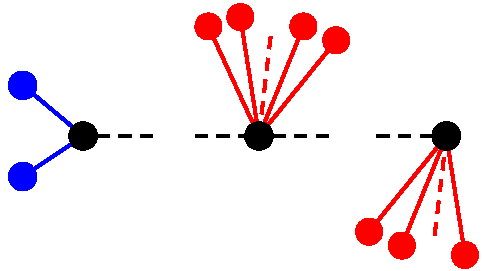
\includegraphics[scale=0.47]{figures/buildtree.pdf}
\caption{\footnotesize Un generico albero $A$ costruito da $d$. Le foglie blu ricordano che $A$ deve contenere almeno due foglie; il cammino iniziale, lungo $k$, è in nero; le foglie rimanenti sono rosse.}
\end{figure}


\section{Un esercizio d'esame sullo score: dall'inizio alla fine}
Si dica, motivando la risposta, quale dei seguenti
vettori è lo score di un grafo e, in caso affermativo,
si costruisca un tale grafo utilizzando il teorema dello score.
\[ d_1=(3,4,4,5,5,5,5,5) \qquad d_2=(2,3,3,3,3,4,5,7,7,7,12,12,12) \]
Si dica inoltre se
\begin{enumerate}
    \item esiste un tale grafo che sia un albero;
    \item esiste un tale grafo che sia hamiltoniano;
    \item esiste un tale grafo che sia sconnesso.
\end{enumerate}
\textit{Soluzione:} non esiste alcun grafo $G$ che
abbia score $d_2$. Infatti, $d_2$ imporrebbe a $G$
di avere 13 vertici dei quali tre di grado 12,
dunque adiacenti a tutti gli altri vertici; allora
il vertice di grado minimo in $G$ dovrebbe avere
almeno grado 3, ma questo contraddice quanto
previsto in $d_2$, dove l'entrata minima equivale
a 2.

Non avendo trovato ostruzioni all'esistenza di
grafi con score $d_1$, procediamo applicando il
teorema dello score a $d_1$. Ciò è possibile
dal momento che $d_{1_8} = 5 \leq 8 - 1$.

\begin{center}
    \begin{tabular}{c|llllllll}
        $d_1$   & 3 & 4 & 4 & 5 & 5 & 5 & 5 & \textcolor{blue}{5}\\
        \hline
        $d_1'$  & 3 & 3 & 4 & 4 & 4 & 4 & \textcolor{orange}{4} & $\times$\\
        \hline
        $d_1''$ & 3 & 3 & 3 & 3 & 3 & \textcolor{red}{3} & $\times$ &\\
        \hline
        $d_1'''$ & 2 & 2 & 2 & 3 & \textcolor{green}{3} & $\times$ &&\\
        \hline
        $d_1''''$ & 1 & 1 & 2 & 2 & $\times$ &&&
    \end{tabular}
\end{center}
Notiamo che da $d_1''''$ è possibile costruire un possibile rispettivo
grafo $G''''$ mostrato di seguito:
\begin{figure}[H]
\centering
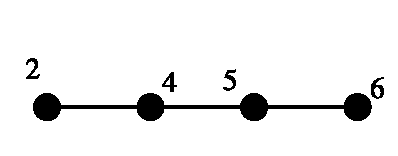
\includegraphics[scale=0.65]{figures/bassefinal.pdf}
\end{figure}

\noindent Per il teorema dello score, allora anche tutti gli altri vettori,
incluso $d_1$, sono lo score di qualche grafo. Costruiamo un grafo
$G$ (si veda la Figura \ref{final}) con score $d_1$ mediante il teorema dello score.
\begin{figure}[H]
\centering
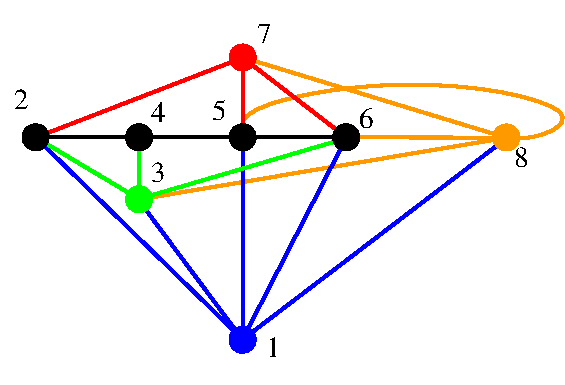
\includegraphics[scale=0.65]{figures/build.pdf}
\caption{$G$}
\label{final}
\end{figure}

\noindent Rispondiamo ora agli altri quesiti:
\begin{enumerate}
    \item Osserviamo che $d_1$ non soddisfa la formula di Eulero:
    \[ 8-1 = 7 \not= \frac{3+4+4+5+5+5+5+5}{2} = 18 \]
    pertanto non esistono alberi con score $d_1$. D'altra parte
    $d_1$, che contiene $8\geq2$ elementi, non possiede nessuna
    entrata pari a 1, ovvero non possiede almeno 2 foglie
    (condizione necessaria all'esistenza di un albero).
    \item Si noti che il ciclo $c=(1,2,3,4,5,6,7,8)$, evidenziato in
    Figura \ref{lasthamiltonian}, in $G$ è hamiltoniano.
    \begin{figure}[H]
    \centering
    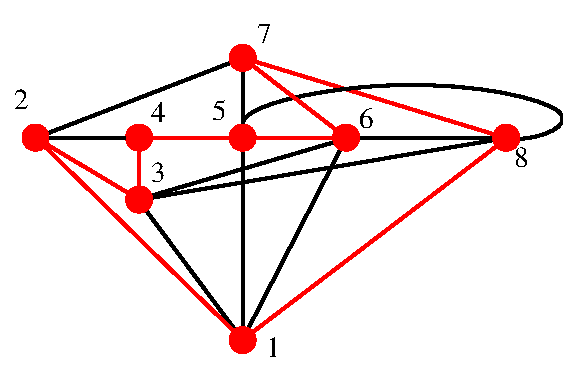
\includegraphics[scale=0.65]{figures/lasthamiltonian.pdf}
    \caption{Un ciclo ($c$) hamiltoniano in $G$.}
    \label{lasthamiltonian}
    \end{figure}
    dunque $G$ è un grafo hamiltoniano con score $d_1$.

    \item Applicando la condizione di \textit{forzatura alla connessione}
    giungiamo alla seguente conclusione:
    \[ 5+3 = 8 > 7 = 8-1 \]
    che soddisfa la forzatura; ma allora ogni grafo con score
    $d_1$ è necessariamente connesso e pertanto non esistono
    grafi sconnessi con score $d_1$.
\end{enumerate}